% fancytikzposter.tex, version 2.1
% Original template created by Elena Botoeva [botoeva@inf.unibz.it], June 2012
% 
% This file is distributed under the Creative Commons Attribution-NonCommercial 2.0
% Generic (CC BY-NC 2.0) license
% http://creativecommons.org/licenses/by-nc/2.0/ 


\documentclass{a0poster}

\usepackage{fancytikzposter} 
\usepackage{fancySettings} 
\usepackage{mystyle}

%%%%%%%%%%%%%%%%%%%%%%%%%%%%%%%%%%%%%%%%%%%%%%%%%%%%%%%%%%%%%%%%%%%%%%%%%%%%%%%%%%%%%%%%%%%%%%%%%%%%%%%%%%%%%%%%%%%%%%%%%%%%%%%%%%%%%%%%%%%%%%%%%%%%%%%%%%%%%%%%%%%%%%%%%%%%%%%%%%%%%%%%%%%%%%

\title{Parallel Tempering \qquad }
\author{ dr Błażej Miasojedow \and \udot{mgr Mateusz Łącki} \\
  Wydział Matematyki, Informatyki i Mechaniki\\ University of Warsaw, Poland\\
  \texttt{B.Miasojedow@mimuw.edu.pl} \\
  \texttt{mateusz.lacki@biol.uw.edu.pl}
}

\usetemplate{1}

\begin{document}

\ClearShipoutPicture
\AddToShipoutPicture{\BackgroundPicture}

\noindent % to have the picture right in the center
\begin{tikzpicture}
  \initializesizeandshifts
  % \setxshift{15}
  % \setyshift{2}


  %% the title block, #1 - shift, the default value is (0,0), #2 - width, #3 - scale
  %% the alias of the title block is `title', so we can refer to its boundaries later
\ifthenelse{\equal{\template}{1}}{ 
  \titleblock{47}{1}
}{
  \titleblock{47}{1.5}
}


  %% #1 - anchor relative to the title block, #2 - shift, #3 - width, #3 - file name
\addlogo[south west]{(2,1.5)}{8cm}{img/logoUniversityOfWarsaw.png}
% \addlogo[south east]{(-2,1.5)}{16cm}{img/logoMimuw.png}


%%%%%%%%%%%%%%%%%%%%%%%%%%%%%%%%%%%%%%%%%%%%%%%%%%%%%%%%%%%%%%%%%%%%%%%%%%%%%%%%%%%%%%%%%%%%%%%%%%%%%%%%%%%%%%%%%%%%%%%%%%%%%%%%%%%%%%%%%%%%%%%%%%%%%%%%%%%%%%%%%%%%%%%%%%%%%%%%%%%%%%%%%%%%%%


\blocknode{Bayesian Modelling for Bioinformatics}{
  \coloredbox{colorthree!50!}
  {\centering Applications}
  \bi
    \item{ Hierarchical modelling for identification of co-expression patterns in microarray
data by cluster analysis \citep{Medvedovic, STING2010} }

    \item{ Assessing the importance of explanatory variables \citep{STING2010} }

    \item{ Model Selection }
  \ei
  \coloredbox{colorthree!50!}{\centering \mcmc}
  \bi
    % \item{ Closed formulas exist only in very restricted case of considering conjugate priors }

    \item{ \mcmc\, algorithms are used to simulate samples out of analytically untractable posterior distributions }
    \bi
      \item{ Most popular algorithm: \GreenMetropolisHastings\, \citep{Geyer}}
      \item{ Generates a sequence of points that are thought of as being an instantiation of a Markov Chain $$X \equiv \{ X^{[k]}\}_{k = 0}^\infty$$  }
      \item{ Approximates, thanks to Ergodic Theory, integrals 
        $$\expect g(X) = \int_\Omega g(x) \mathrm{d}\,\pi \approx \frac{1}{\nn}\sum_{i = 1}^\nn g(X^{[i]}),$$
        where $\pi$ is the requested a posteriori distribution. In particular: we can approximate probabilities of any measurable set, $\prob{(A)}$
       }
    \ei

    \item{ \GMH\,estimates may suffer from poor mixing}
    \bi
      \item{ Chain $X$ restricted to user-provided number of iterations $\nn$ could get stuck in a probability cluster }
      \item{ Multimodial priors result in multimodial posteriors }
      \item{ Multimodial priors are selected when we suspect that the phenomenon under study is not concentrated around a particular point }
    \ei
  \ei  

   \coloredbox{colorthree!50!}{\centering Example} 

  \begin{center}
    \begin{tabular}[t]{cc}
      \begin{minipage}{0.25\linewidth}
        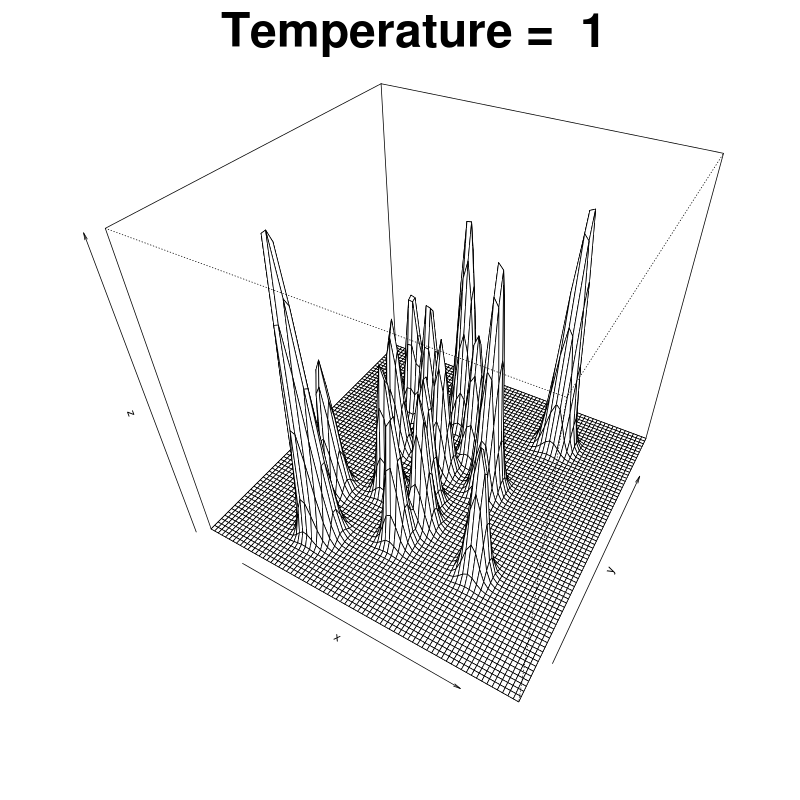
\includegraphics[width=1\textwidth]{img/Liang_perspective.png}
      \end{minipage}
      & 
      {\small \begin{minipage}{0.75\linewidth}
        \bi 
          \item{ Consider $\pi$ given by density $f$ that is a mixture of normal distributions
            \begin{equation*}
              f(x) = 
              \sum_{i=1}^{20} \frac{\omega_i}{ \sigma_i \sqrt{2 \pi} } \exp \Big( -\frac{(x - \mu_i)^\tran (x - \mu_i)}{2 \sigma_i^2} \Big)  
            \end{equation*} 
            where $\sigma_i$ are standard deviations, $\omega_i$ are weights, and $\mu_i$ are means.
          }
          \item{Some of the peaks mingle together to form bigger ones}
        \ei  
      \end{minipage}}
    \end{tabular}
  \end{center}

  \begin{center}
    \begin{tabular}[t]{cc}
      {\small \begin{minipage}{0.75\linewidth}
        \bi 
          \item{ 
            \GMH\, draws sample points from only two modes   
          }
          \item{
            Estimates of probabilities and moments are totally fallacious
          }
        \ei  
      \end{minipage}}
      &
      \begin{minipage}{0.25\linewidth}
        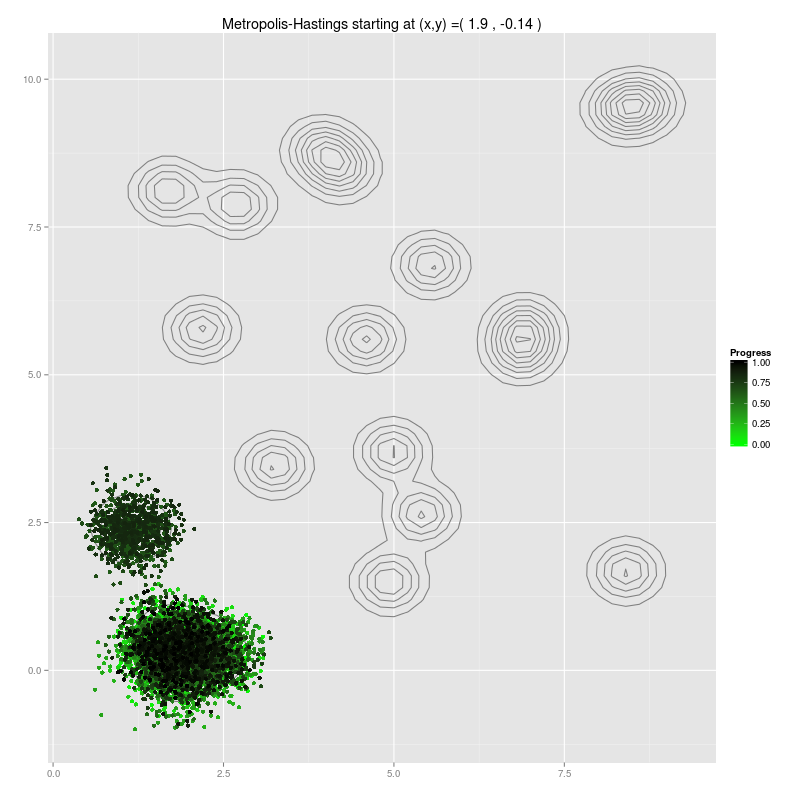
\includegraphics[width=.75\textwidth]{img/MH_simululation_10000_steps.png}
      \end{minipage} 
    \end{tabular}
  \end{center}
}

\coordinate (hello) at ($(currenty)$);

%%%%%%%%%%%%%%%%%%%%%%%%%%%%%%%%%%%%%%%%%%%%%%%%%%%%%%%%%%%%%%%%%%%%%%%%%%%%%%%%%%%%%%%%%%%%%%%

\blocknode[($(currenty)-(0,3)$)]{Parallel Tempering}{   
Hello.
}

%%%%%%%%%%%%%%%%%%%%%%%%%%%%%%%%%%%%%%%%%%%%%%%%%%%%%%%%%%%%%%%%%%%%%%%%%%%%%%%%%%%%%%%%%%%%%%%


\plainblock[-5]{($(hello)+(0,3)$)}{30}{?`Question?} %
{
  \vspace{0.3cm}\\
  How can we enhance mixing so that the \textsc{State Space} is better searched for probability clusters? 
}


%%%%%%%%%%%%%%%%%%%%%%%%%%%%%%%%%%%%%%%%%%%%%%%%%%%%%%%%%%%%%%%%%%%%%%%%%%%%%%%%%%%%%%%%%%%%%%%



% \blocknode[($(currenty)-(0,15)$)]{Parallel Tempering}{   
% Hello.
% }



% \blocknode[($(currenty)-(0,15)$)]{Fallacious Inferences}{   
%   \begin{tikzfigure}
%     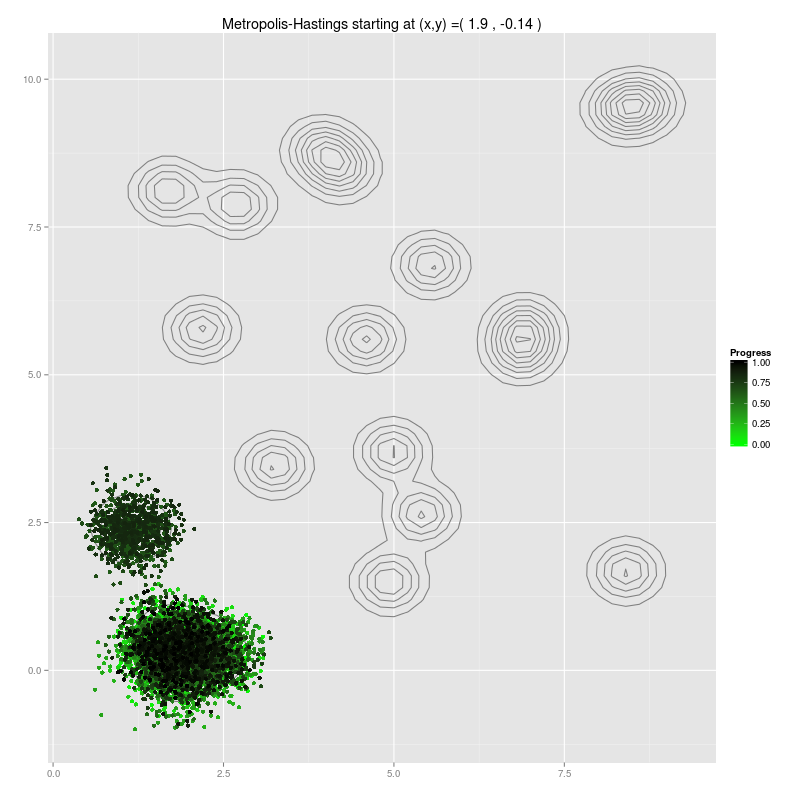
\includegraphics[scale=.2]{img/MH_simululation_10000_steps.png}
%   \end{tikzfigure}  
% }

% \blocknode{Picture}{
%   \begin{tikzfigure}[Metropolis Hastings]
    % 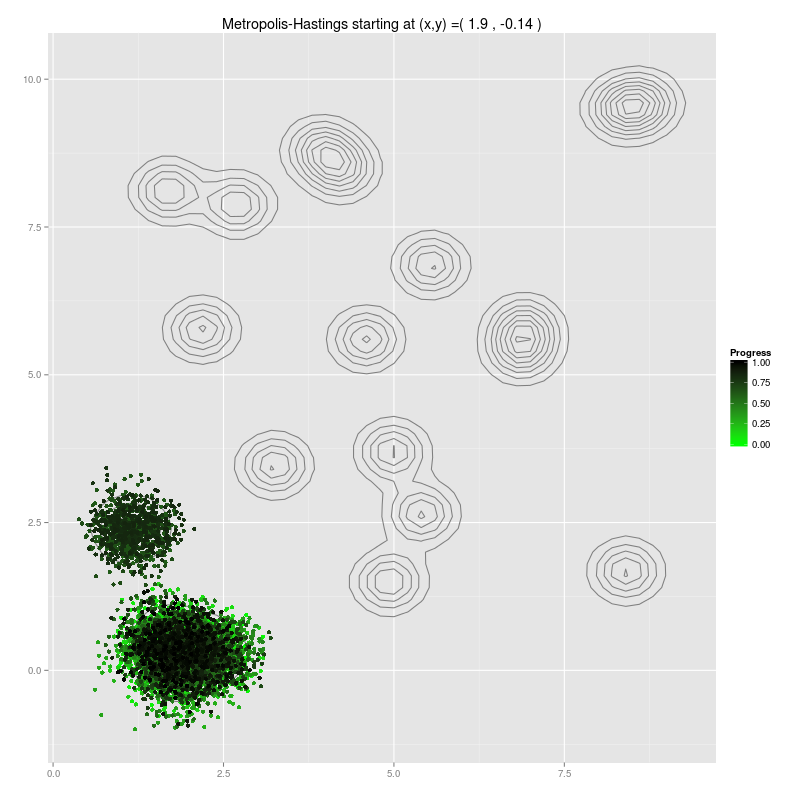
\includegraphics[scale=.3]{img/MH_simululation_10000_steps.png}
%   \end{tikzfigure}
% } 







%%%%%%%%%%%%%%%%%%%%%%%%%%%%%%%%%%%%%%%%%%%%%%%%%%%%%%%%%%%%%%%%%%%%%%%%%%%%%%%%%%%%%%%%%%%%%%%%%%%%%%%%%%%%%%%%%%%%%%%%%%%%%%%%%%%%%%%%%%%%%%%%%%%%%%%%%%%%%%%%%%%%%%%%%%%%%%%%%%%%%%%%%%%%%%

\startsecondcolumn
\blocknode{Hug Multimodiality}{Parallel Tempering rocks}



%%%%%%%%%%%%%%%%%%%%%%%%%%%%%%%%%%%%%%%%%%%%%%%%%%%%%%%%%%%%%%%%%%%%%%%%%%%%%%%%%%%%%%%%%%%%%%%%%%%%%%%%%%%%%%%%%%%%%%%%%%%%%%%%%%%%%%%%%%%%%%%%%%%%%%%%%%%%%%%%%%%%%%%%%%%%%%%%%%%%%%%%%%%%%%

\startthirdcolumn
\blocknode{Bye}{
bkas
  Bye World \citet{Medvedovic}
    Bye World \citet{Baragatti}
      Bye World \citet{Miasojedow}
}

\blocknode{References}{
  \bibliographystyle{bibliography/eccaNoNotes}
  \tiny{ 
    \bibliography{bibliography/references}
  }
}

\end{tikzpicture}


\end{document}



%%%%%%%%%%%%%%%%%%%%%%%%%%%%%%%%%%%%%%%%%%%%%%%%%%%%%%%%%%%%%%%%%%%%%%%%%%%%%%%%%%%%%%%%%%%%%%%%%%%%%%%%%%%%%%%%%%%%%%%%%%%%%%%%%%%%%%%%%%%%%%%%%%%%%%%%%%%%%%%%%%%%%%%%%%%%%%%%%%%%%%%%%%%%%%%%%%%%%%%%%%%%%%%%%%%%%%%%%%%%%%%%%%%%%%%%%%%%%%%%%%%%%%%%%%%%%%%%%%%%%%%%%%%%%%%%%%%%%%%%%%%%%%%%%%%%%%%%%%%%%%%%%%%%%%%%%%%%%%%%%%%%%%%%%%%%%%%%%%%%%%%%%%%%%%%%%%%%%%%%%%%%%%%%%%%%%%%%%%%%%%%%%%%%%%%%%%%%%%%%%%%%%%%%%%%%%%%%%%%%%%%%%%%%%%%%%%%%%%%%%%%%%%%%%%%%%%%%%%%%%%%%%%%%%%%%%%%%%%%%%%%%%%%%%%%%%%%%

% \plainblock[5]{($(currenty)+(-5,0)$)}{26}{Multimodial Example} %
% {
%   \vspace{0.3cm}\\
%   Consider $\pi$ given by density $f$ that is a mixture of normal distributions
%   \begin{equation*}
%     f(x) = 
%     \sum_{i=1}^{20} \frac{\omega}{ \sigma \sqrt{2 \pi} } \exp \Big( -\frac{(x - \mu_i)^\tran (x - \mu_i)}{2 \sigma^2} \Big),  
%   \end{equation*}
%   s.t. $\sigma = 0.1$, $\omega = 0.05 $, with means 

%   {
%     \centering
%     \tiny{
%       \begin{tabular}{rrrrrrrrrrrrrrrrrrrr}
%         \hline
%       $\mu_1$ & $\mu_2$ & $\mu_3$ & $\mu_4$ & $\mu_5$ & $\mu_6$ & $\mu_7$ & $\mu_8$ & $\mu_9$ & $\mu_{10}$ & $\mu_{11}$ & $\mu_{12}$ & $\mu_{13}$ & $\mu_{14}$ & $\mu_{15}$ & $\mu_{16}$ & $\mu_{17}$ & $\mu_{18}$ & $\mu_{19}$ & $\mu_{20}$ \\ 
%         \hline
%       2.18 & 8.67 & 4.24 & 8.41 & 3.93 & 3.25 & 1.70 & 4.59 & 6.91 & 6.87 & 5.41 & 2.70 & 4.98 & 1.14 & 8.33 & 4.93 & 1.83 & 2.26 & 5.54 & 1.69\\ 
%         5.76 & 9.59 & 8.48 & 1.68 & 8.82 & 3.47 & 0.50 & 5.60 & 5.81 & 5.40 & 2.65 & 7.88 & 3.70 & 2.39 & 9.50 & 1.50 & 0.09 & 0.31 & 6.86 & 8.11\\ 
%          \hline
%       \end{tabular}
%     }
%   }
% }
